\section*{Problem 6}

Consider the following sampling and reconstruction configuration:

\begin{figure}[H]
\caption*{}
\centering
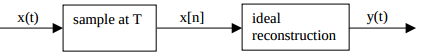
\includegraphics[width=0.7\textwidth]{figs/c3p31.png}
\label{fig:c3p31}
\end{figure} 

The output y(t) of the ideal reconstruction can be found by sending the sampled signal 
$x_s(t) = x(t)p(t)$ through an ideal lowpass filter:

\begin{figure}[H]
\caption*{}
\centering
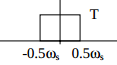
\includegraphics[width=0.2\textwidth]{figs/c3p32.png}
\label{fig:c3p32}
\end{figure} 

\begin{itemize}
\item Let $x(t) = 1 + cos(15\pi t)$ and T = 0.1 sec.
Draw $|X_s(\omega)|$ where $x_s(t) = x(t)p(t)$. 
Determine the expression for y(t).
\end{itemize} 

\subsection*{Solution}

First we calculate $X(\omega)$.

\begin{equation*}
\begin{aligned}
X(\omega) &= \pi [ 2 \delta(\omega) + 
	\delta(\omega - 15\pi) + \delta(\omega + 15 \pi)] 
\end{aligned}
\end{equation*} 

The plot of the magintude of $X(\omega)$ is:
\zcodemat{sources/c3p6a1.m}{Plot of Magnitude}

\begin{figure}[H]
\caption{Magnitude $|X(\omega)|$}
\centering
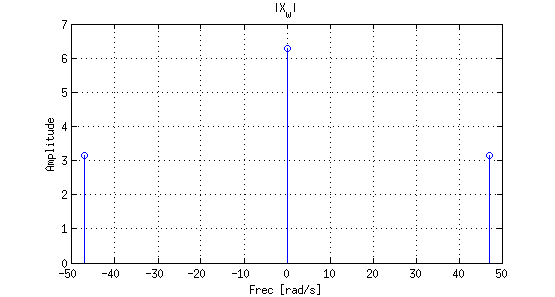
\includegraphics[width=0.8\textwidth]{figs/c3p6a1.png}
\label{fig:c3p6a1}
\end{figure} 

The minimum sampling period of the signal according to the Nyquist theorem is:

\begin{equation*}
\begin{aligned}
\omega_m &= 15 \pi \\
\omega_{Ns} >&= 2 \omega_m >= 30 \pi \\
T_{Ns} &= \frac{2 \pi}{\omega_s} <= \frac{1}{15} <= 0.066
\end{aligned}
\end{equation*} 

Since $T_s = 0.1 sec$ is greater than the minimum required,
aliasing will occur as can be seen in (\ref{fig:c3p6a2}).

\begin{equation*}
\omega_s = \frac{2 \pi}{T_s} =  20 \pi
\end{equation*} 

\zcodemat{sources/c3p6a2.m}{Plot of $|X_s(\omega)|$}

\begin{figure}[H]
\caption{Sampling $|X_s(\omega)|$}
\centering
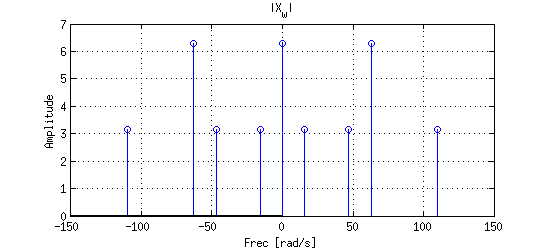
\includegraphics[width=0.8\textwidth]{figs/c3p6a2.png}
\label{fig:c3p6a2}
\end{figure}

The limits of the lowpass filter are $-0.5 \omega_s = -10 \pi$ to $0.5 \omega_s = 10 \pi$.
The Fourier transform of $Y(\omega) = H(\omega)X(\omega)$ is:

\begin{figure}[H]
\caption{Magnitude $|X(\omega)|$}
\centering
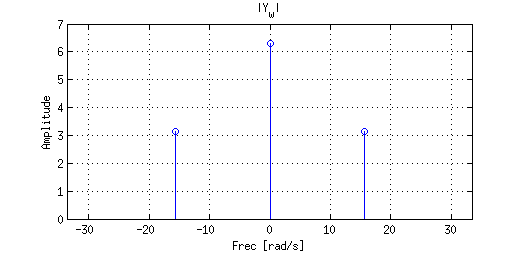
\includegraphics[width=0.8\textwidth]{figs/c3p6a3.png}
\label{fig:c3p6a3}
\end{figure}

And therefore only the $\omega = 5 \pi$ passes through it:

\begin{equation*}
\begin{aligned}
y(t) = 1 + cos(5 \pi t)
\end{aligned}
\end{equation*} 

%%%%%%%%%%%%%%%%%%%%%%%%%  B  %%%%%%%%%%%%%%%%%%%%%%%%%%%%
\begin{itemize}
\item Let $X(\omega) = \frac{1}{(j\omega+1)}$ and T = 1 sec.
Draw $|X_s(\omega)|$ where $x_s(t) = x(t)p(t)$. 
Does aliasing occur? (Justify your answer).
\end{itemize} 

\subsection*{Solution}

The magnitude of $X(\omega)$ is:
\begin{equation*}
\begin{aligned}
|X(\omega)| = \frac{1}{\omega^2 + 1}
\end{aligned}
\end{equation*} 

From the previous equation we can see that the function never intesects the w axis,
and therefore there will always be aliasing. 
However, setting $w_m$ to its FWHM we have:

\begin{equation*}
\begin{aligned}
\frac{1}{\omega_m^2+1} &= \frac{1}{2} \\
\omega_m = \sqrt{3}
\end{aligned}
\end{equation*} 

Hipoteticaly taking this value as $w_m$ we see that 
$w_s = 2 \pi > 2 w_m = 2 \sqrt{3} $ and in this case there will
not be aliasing.

The plot of the magintude of $X(\omega)$ and $X_s(\omega)$ is:
\zcodemat{sources/c3p6b1.m}{Plot of Magnitude}

\begin{figure}[H]
\caption{Magnitude}
\centering
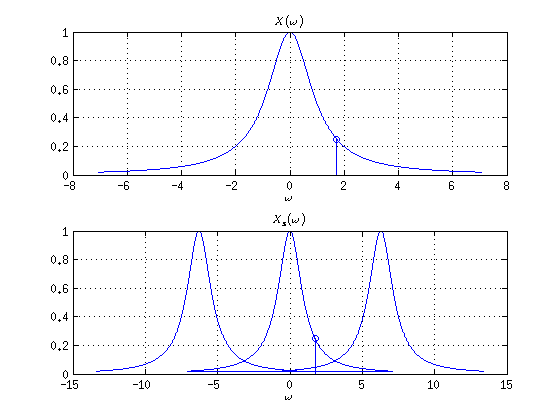
\includegraphics[width=0.8\textwidth]{figs/c3p6b2.png}
\label{fig:c3p6b2}
\end{figure} 

